\section{Введение}
\label{sec:Chapter0} \index{Chapter0}

Одно из активно развивающихся направлений в сфере машинного обучения является трансляция доменов. Данная задача состоит в нахождении трансляции (отображении) $G$, которое переносит элементы одного домена, $X$, в другой, $Y$. Например, трансляция синтетических изображения с камеры видео-регистратора в реальные (рисунок \ref{fig:domains-example}). 

\begin{figure}
    \centering
    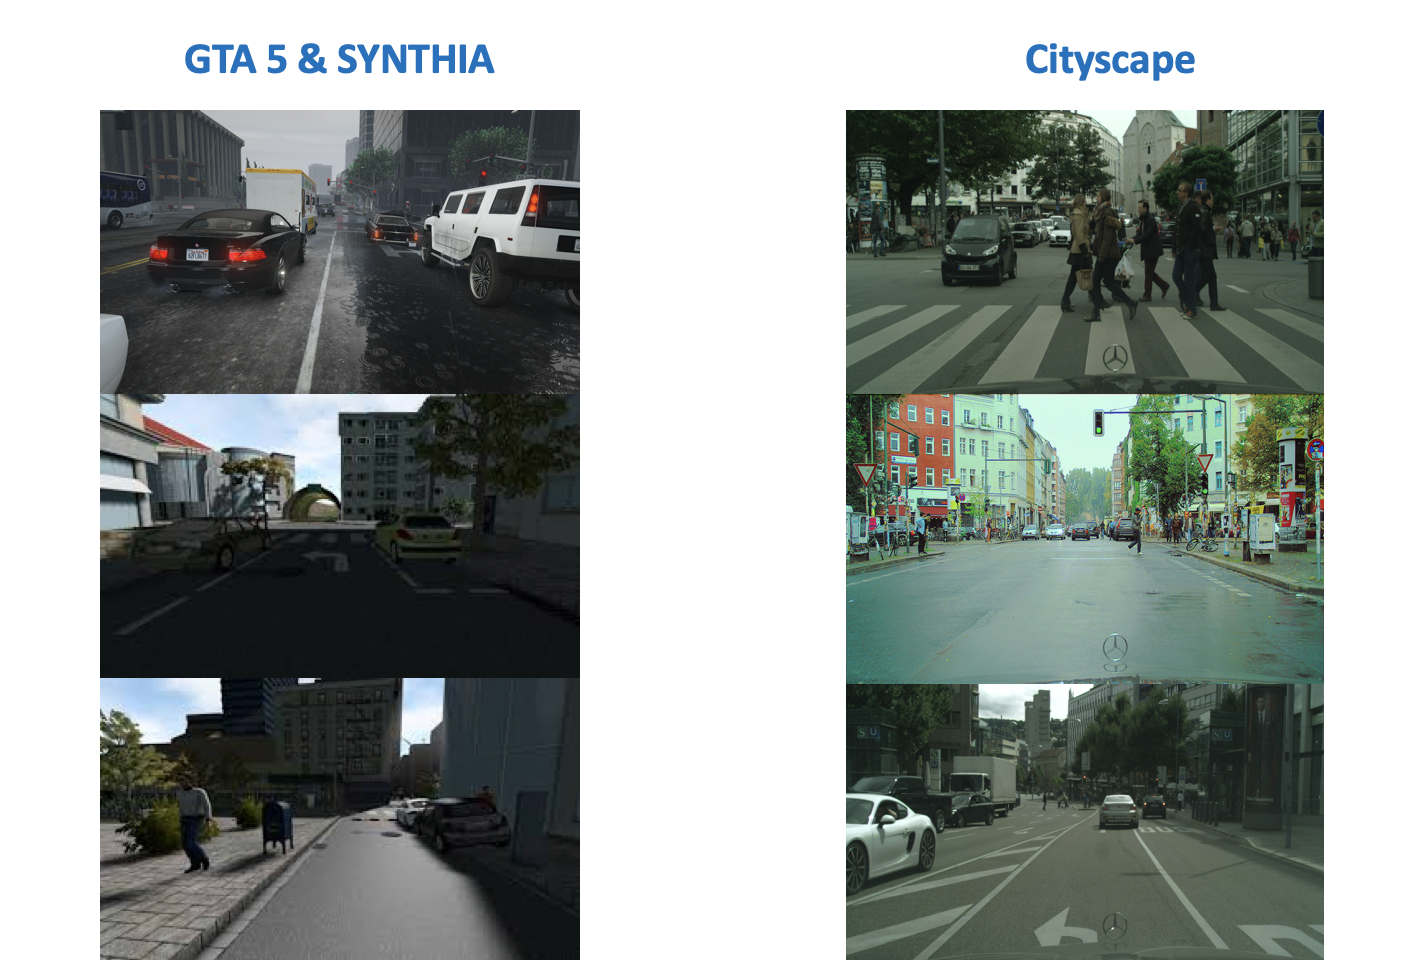
\includegraphics[scale=0.3]{images/domains_example.png}
    \caption{Два домена: синтетические и реальные виды города}
    \label{fig:domains-example}
\end{figure}

Сильным развитием данной задачи послужила, частная формулировка трансляции домена, а именно генеративное моделирование. Пусть дан наблюдаемый набор данных $Y$, элементы, $y$, которого принадлежат базовому распределению $y \sim \pi_y$. Цель любой генеративной модели состоит в том, чтобы аппроксимировать это распределение данных при наличии доступа к $Y$. После обучения, такая модель позволяет генерировать новые объекты $\hat y \notin Y$.

Так, например, состязательные сети (GAN), предложенные Гудфуллоу в статье \cite{gan}, стали основой одного из значимых методов в задаче трансляции домена. В GAN обучается две модели генератор и дискриминатор, первая из которых пытается сгенерировать реалистичные данные, а вторая пытается определить, является ли данные реальными или сгенерированными. Разработанный подход позволяет обучать неявным образом генеративные распределения, используя только сэмплы из реального распределения данных $p_y$. Методом, который обобщает GAN на задачу трансляции доменов, является CycleGAN, предложенный в \cite{cycle-gan}. Данный метод обучает два GAN, которые отображают данные в элементы противоположного набора.

Следующий класс генеративных моделей, адаптированных на задачу трансляции домена, стали диффузионные модели \cite{ddpm}. Они полагаются на итеративную процедуру, при которой распределение данных $p_{data}$ сначала искажается с помощью процесса прямого зашумления, сходящегося к нормальному распределению. Затем изучается обратный во времени процесс, который восстанавливает данные из гауссовского распределения обратно в распределение данных, с использованием score matching подходов. Для обобщения данной задачи важную роль сыграло понимание ограничений, а именно фиксированного нормального распределения, которое является не самым оптимальным выбором скрытого пространства. Например, для задачи восстановления зашумленных изображение, имея соответсвующее изображение высокого качества, имеет смысл восстанавливать начиная с зашумленного. Однако, это требует изменения целевого распределения прямого процесса, что часто неразрешимо и приводит к численным трудностям. 

В качестве обобщения диффузионных моделей на задачу трансляции домена был предложен метод Bridge matching \cite{bridge-matching}. Аналогично с диффузионными моделями данный метод, строит два стохастических процесса, прямой и обратный, между двумя маргинальными распределениями, таким образом обобщая задачу на два заданные произвольные распределения.

Однако вышеуказанны подходы обладают рядом недостатков. Во-первых, для Bridge matching требуются специализированные наборы данных, объекты которых являются пары из двух заданных конечных распределений, то есть во время обучения оба элемента пары должны соответствовать одному объекту, например, изображение представленное в двух видах: зашумленное и высокого качества. Во-вторых, в данных методах никак не задается оптимальность отображений. В статье \cite{translation-optimality} показывается, что данные методы ориентированы на небольшие преобразования. Это не является проблемой, когда распределения близки друг к другу, но в обратной ситуации, это не позволяет уловить более сложную семантику распределений. Таким образом, возникает потребность внедрять информацию о данных, что требует для каждой задачи адаптировать целевую функцию. 

Решением этих проблем является введение дополнительные критериев оптимальности отображений. Такими требованиями обладают мосты Шрёдингера \cite{schrödinger}, \cite{leonard-survey}. Задача мостов Шрёдингера находит стохастический процесс (рисунок \ref{fig:bridges_example}), ограниченный двумя заданными конечными распределениями, который наиболее похож с винеревским процессом с точки зрения дивергенции Кульбака — Лейблера. Такая формулировка задачи позволяет находить отображения между двумя непарными наборами данных, а также наиболее оптимальным образом, с точки зрения квадрата расстояния между элементами. Кроме того, данная задача позволяет вычислять вероятность этого стохастического процесса, что позволяет нам сравнивать два набора данных, что может быть полезно для проверки гипотез и семантического сходства.

\begin{figure}
    \centering
    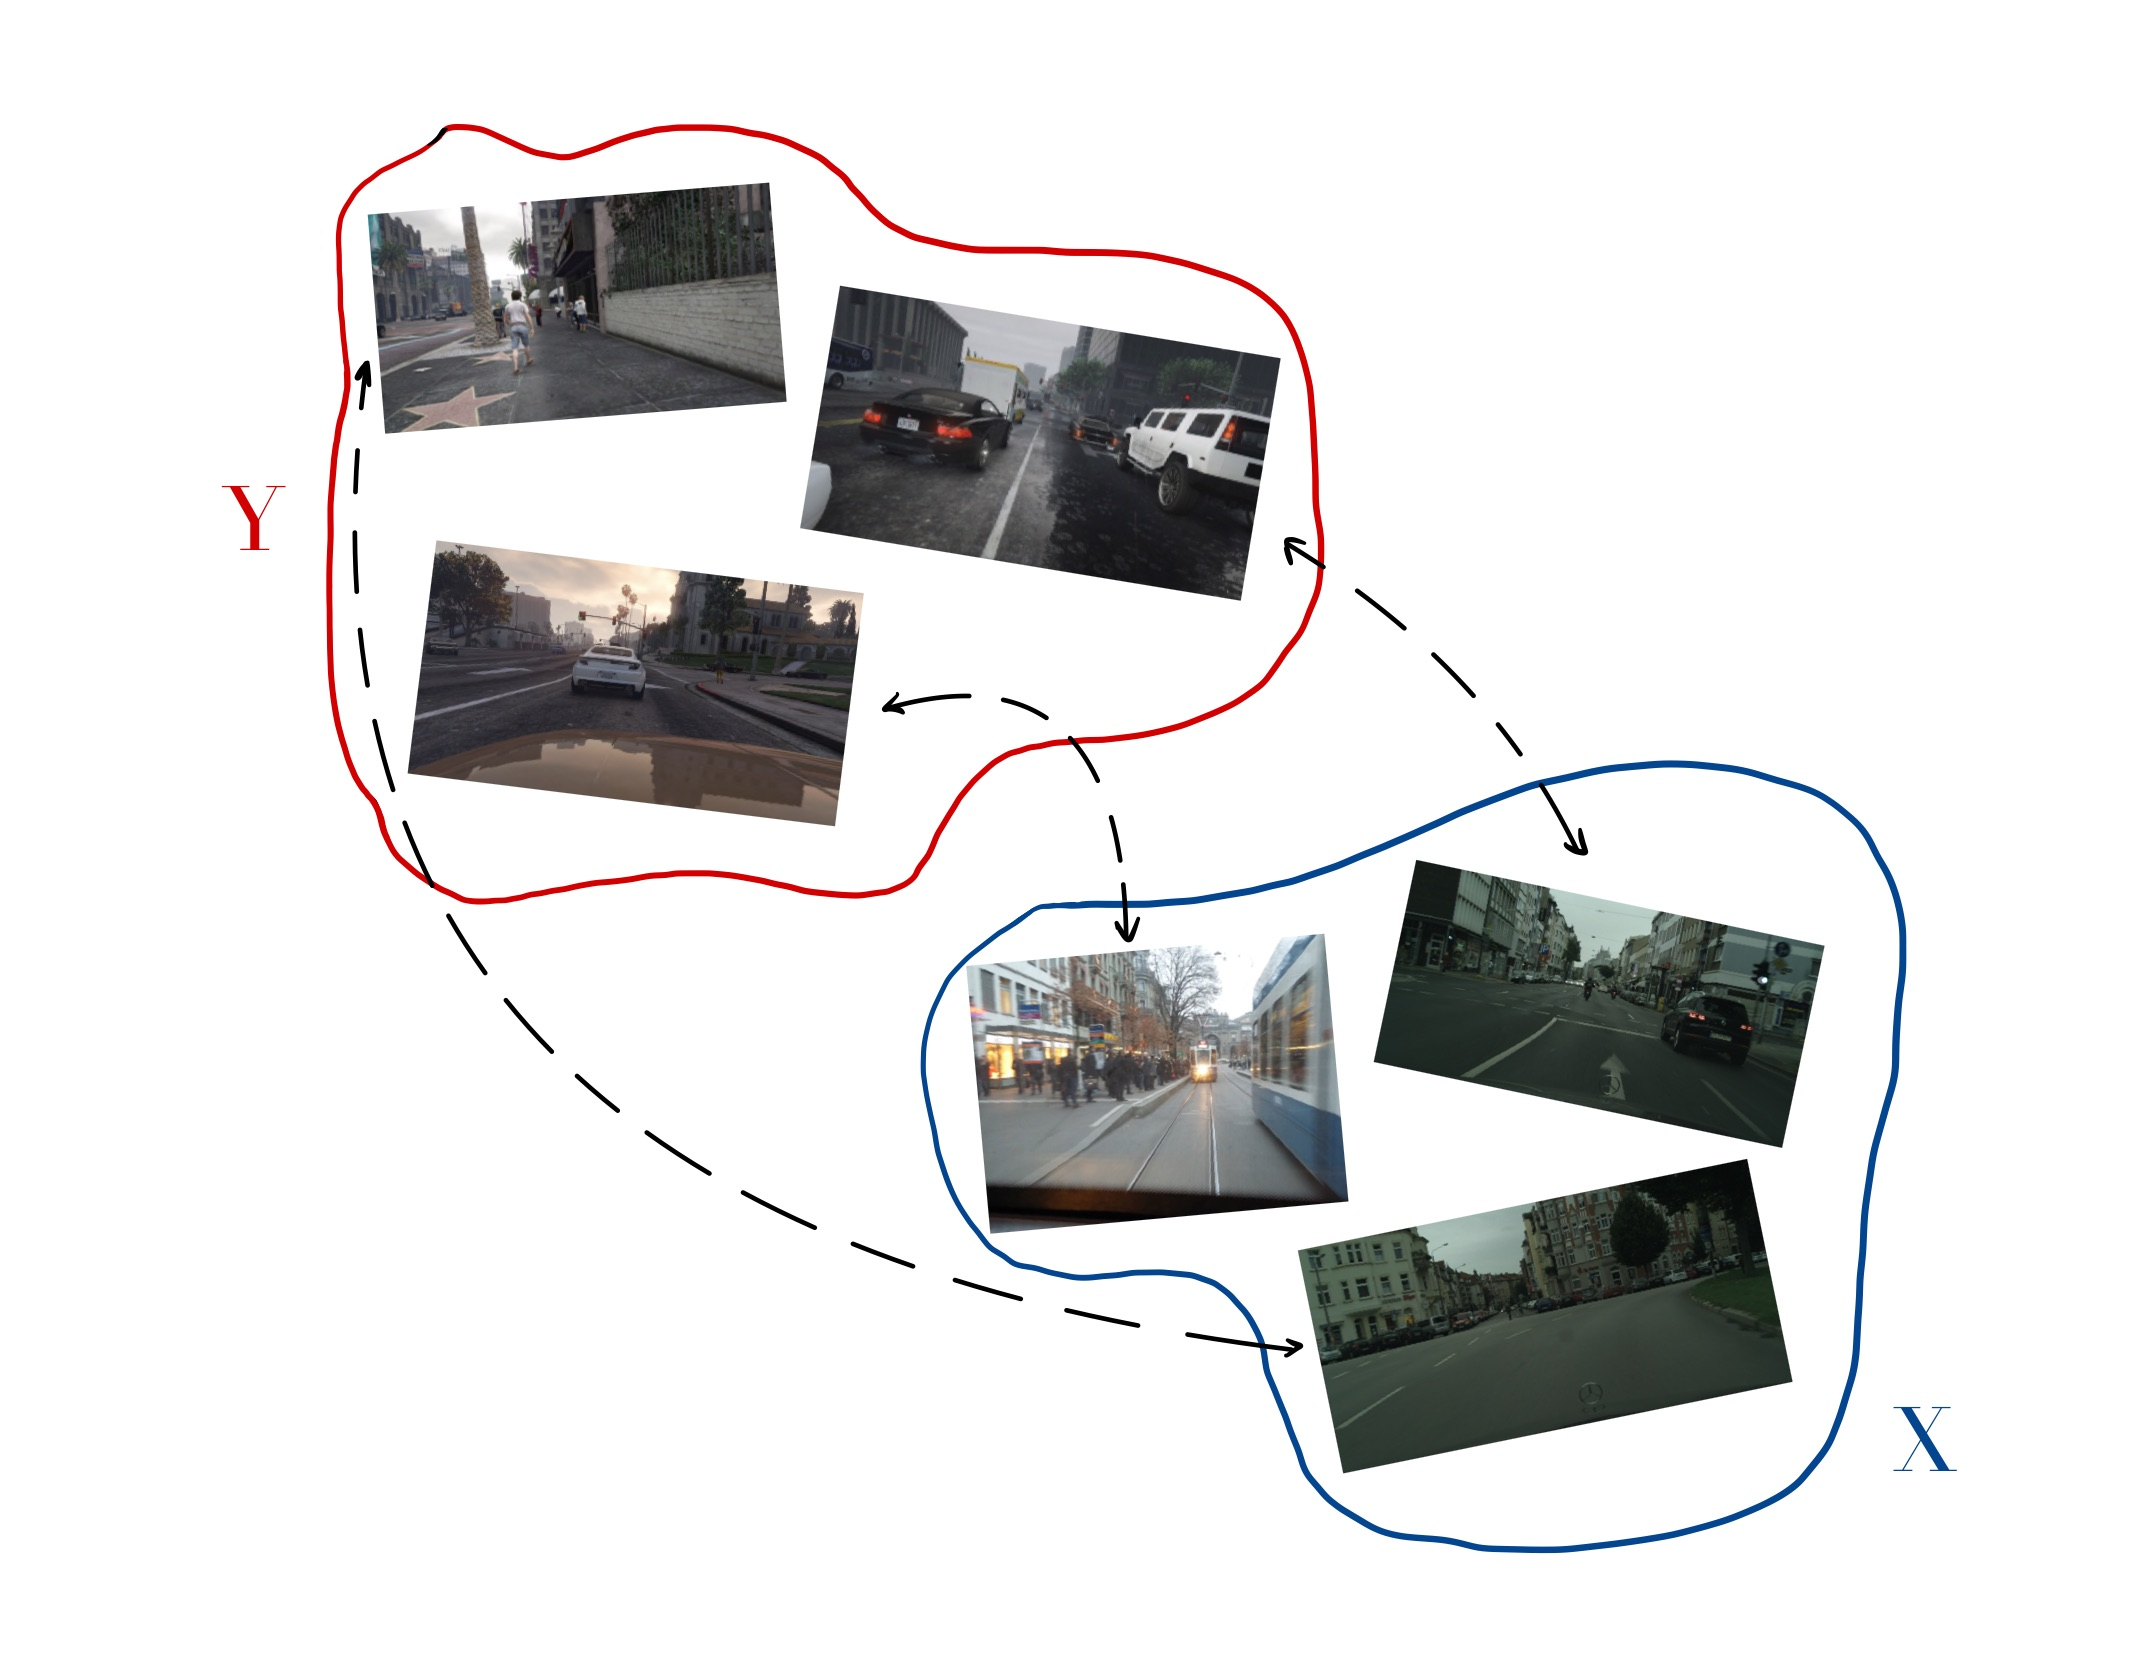
\includegraphics[scale=0.2]{images/bridges_example.jpg}
    \caption{Иллюстрация мостов Шрёдингера}
    \label{fig:bridges_example}
\end{figure}

Также, несомненная актуальность исследований в сфере мостов Шрёдингера подтверждается количеством статей, публикуемых в данное время. Так по запросу сайта arXiv\footnote{https://arxiv.org/} количество статей за последние 12 месяцев составило 56, когда год назад за такой же промежуток времени результат оказался в два раза меньше и составил 23 статьи.

Из-за родства диффузионных генеративных моделей с мостами Шрёдингера было предложено несколько подходов \cite{dsb}, \cite{dsbm}, \cite{mle-sb}, \cite{cycle-sb}. Несмотря на качество полученных результатов подходы предложенные в этих статьях являются вычислительно-дорогостоящими из-за этого возникает потребность в использовании других методов построения мостов Шредингера. 

Одними из примеров работ, которые не обладают данной проблемой, являются подходы описанные в следующих статьях \cite{lsb} и \cite{pavon-empiric-fortret}. Однако данные методы обладают другой проблемой: они страдают от проклятия размерности. Первый, несмотря на значительную скорость обучения, не предназначен для работы с такими данными. А второй метод, из-за особенностей оценивания интеграла, становится сложно вычислимым для данных большой размерности.

Благодаря исследованиям состязательных генеративных сетей \cite{fgan}, а именно доказательству, что целевая функция GAN может быть обобщена до f-семейства дивергенций, в данной работе предлагается новый подход к обучению мостов Шредингера, который наследует преимущества состязательных генеративных сетей и решает вышеперечисленные проблемы.

\newpage
